\chapter{System design}
Since the hardware choice was dictated by the current system base and client choice there is not much to be discussed in this field. This chapter will give just a quick overview of the hardware design and then will concentrate on the software part and in particular drift rate algorithm development.

This project is based on the system that is currently in place, it has control over PTU can take readings from the inclinometer and control relays. It consists of the Gumstix minicomputer, GPIO14 chip, relays, inclinometer, PTU, server side code (running on Gumstix), client side code (provides API for the interaction with the server) and the library implementing PTU TASS communication protocol to interact with the PTU. 

\section{Changes to the system}
There was a decision made by the client to replace the platform (Gumstix) that is currently used. The rationale behind the decision were client's concerns about the currently used Gumstix computer which is getting old. In case of a breakdown it would be difficult to find the replacement parts. One of the features requested was the ability to compile accompanying code on the platform itself (this is currently impossible on the Gumstix due to the hardware limitations) instead of cross-compiling code on the PC and then uploading executables to the Gumstix. Following a thorough discussion Raspberry Pi minicomputer was chosen as a replacement platform. It has enough power to compile the code as well as all the required interfaces for the connection of the other equipment. PTU TASS library will be reused and its functionality extended to implement the new features. Server and client side codes will be adjusted accordingly to provide access to the new functionality.

\section{System architecture overview}
This project will consist from the hardware and software parts, each of them will be discussed further in this chapter. The server side will have software running on the Raspberry PI minicomputer and handling all client requests. Connection will be initiated by the client over the TCP/IP protocol. Client side application will be using provided AberBox API to send/receive commands. Overall system archite cture is presented on the figure ~\ref{fig:SystemArchitectureOverview}.

\begin{figure}[H]
\centering
\centerline{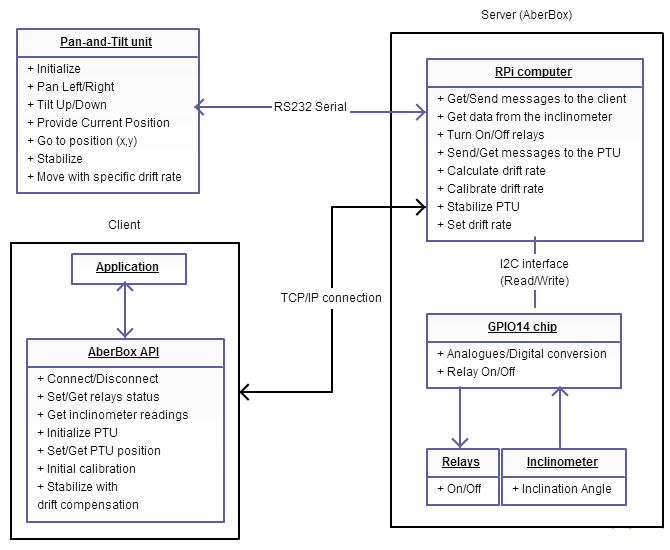
\includegraphics[scale=0.80]{./images/SystemArchitectureOverview}}
\caption{System Architecture Overview}
\label{fig:SystemArchitectureOverview}
\end{figure}

\section{Hardware Design}
The proposed system will consist of the Raspberry Pi minicomputer, analogue inclinometer, GPIO14 chip, relays and the PTU.

\subsection{Raspberry Pi}
As a platform for the main control system Raspberry Pi minicomputer was chosen. It will replace the currently employed for this task Gumstix single board computer. 

Raspberry Pi is a credit-card-sized single-board computer with a 512 MiB of RAM and 700 MHz ARM based CPU. It is powerful enough for the proposed tasks to be completed and have all the required interfaces to be connected to the other peripheral. It has GPIO pins, including SPI and I$^2$C interfaces, UART serial console, 5v and GND supply pins. Since there will be loads of power available on the vehicle power consumptions of the device were not taken in to account when choosing the platform. Such a powerful device may be an overkill for this task, but the decision was made by the client. Furthermore in the future this platform may be used to handle additional tasks.

\subsection{Inclinometer}
An inclinometer will be required to get data about the current chassis position in the space. The client suggested to use the analogue SCA121T-D05 dual axis inclinometer (figure~\ref{fig:SCA121T-D05_inclinometer}) that provided instrumentation grade performance for levelling applications in harsh environment. It will be bolted to the chassis of the vehicle and will provide information about the inclination angles. This data will then be used during the PTU drift rate calibration. Since it is an analogue device a way to convert from analogue to digital format will be required.

\begin{figure}[H]
\centering
\centerline{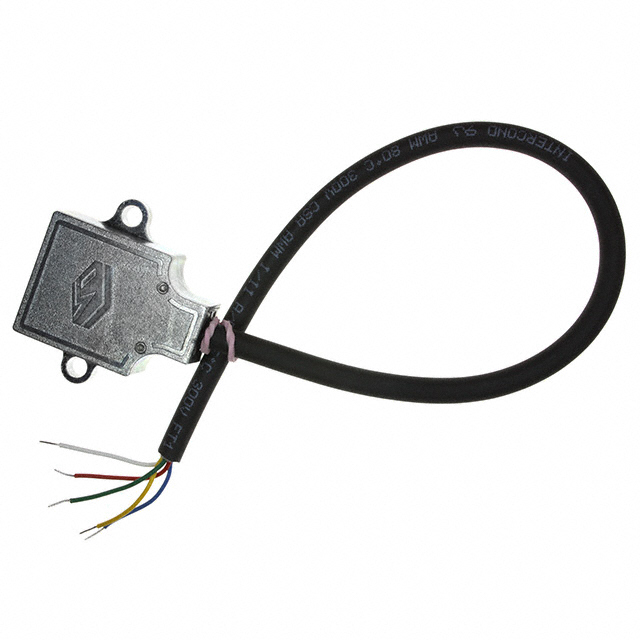
\includegraphics[scale=0.20]{./images/SCA121T}}
\caption{SCA121T-D05 Inclinometer}
\label{fig:SCA121T-D05_inclinometer}
\end{figure}

\subsection{GPIO14 Chip}
The GPIO14 chip is a pre-programmed PIC16F818 micro controller. It intends to provide general purpose I/O expansion on the $I^2$C bus. It has 14 general purpose I/O lines and 5 analogues input channels with 10-bit A/D conversion \cite{GPIO14}. GPIO14 chip will be used to convert inclinometer signal from the analogue format to digital and to switch on/off relays. This chip will be connected over the I$^2$C bus to the Raspberry Pi.

\subsection{PTU}
Pan-and-Tilt Unit is a high-precision integrated motion control systems produced by the Sagebrush Technology (now part of the RIEtech Global, LLC \cite{RIEtech_Global}). It is designed for the <10Kg payloads and is often used to hold cameras, antennas or for instrument positioning. To connect it to the Raspberry Pi (which has TTL interface) RS-232 to TTL converter will be used. As a part of this project it is used to hold a panoramic camera. 

\section{Software Design}
This study will be based on the code that is already used on the Gumstix. It is currently used to send control commands to the PTU, get readings from the inclinometer and switch on/off relays. The code base consists of three main parts: the client side software, the server side software (running on the Gumstix and responding to client calls) and the library that implements PTU TASS communication protocol. In this section different software design aspect will be discussed

\subsection{PTU TASS library}
\label{PTUTASSlibrary}
PTU TASS library is written in the C++ and implements commands to communicate with the PTU. All communication is done over the serial interface. Currently the library has all the necessary commands implemented to perform basics tasks such as: pan left/right, tilt up/down, get/set position, get/set rotation limits. One of the objectives of this project is to implement 'stabilize' and 'drift rate' commands, as well as drift rate calculation. 

The class diagram for the library is presented on the figure ~\ref{fig:PTinterface}. PTinterface class provides functionality to interact with the PTU. It has two data structures defined. PTcoord data structure is used to hold values of the PTU position. DriftRate data structure is created at the beginning of the program and stores drift rate values for the both axes, there is a \texttt{StabilizationTime} attribute as well, it is required to store time of the last call to stabilization command. The drift rate data structure will have \texttt{private} access specifier since it should be accessed by the instantiated object only, no other code should be able to modify values inside since it will affect the PTU drift rate value used for the drift rate cancellation.

\begin{figure}[H]
\centering
\centerline{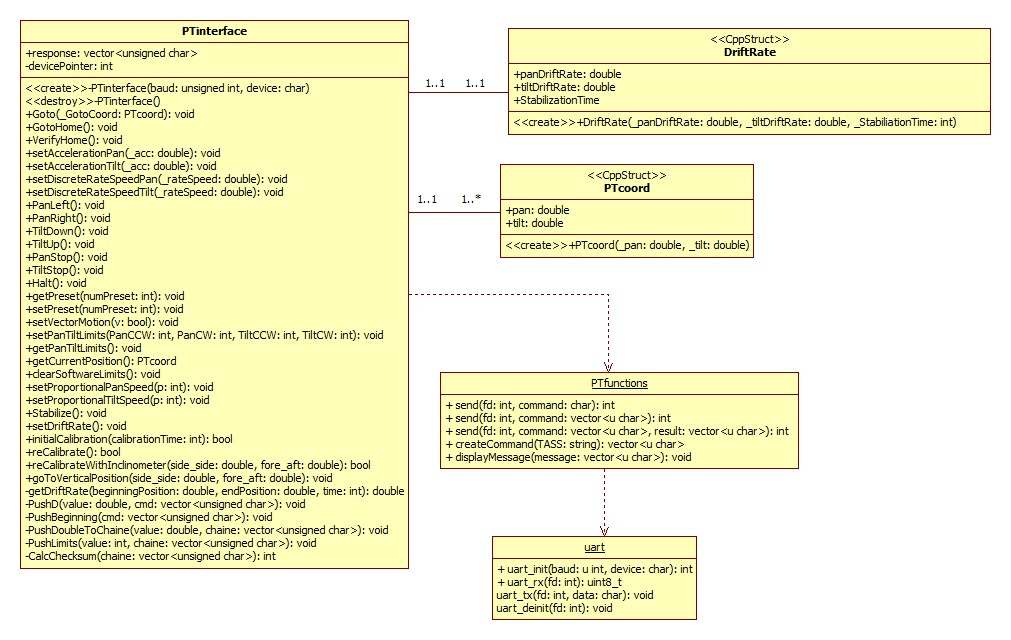
\includegraphics[scale=0.53]{./images/PTinterface}}
\caption{PTU TASS library}
\label{fig:PTinterface}
\end{figure}

\subsubsection{Stabilization command}
The stabilization command tells PTU to maintain a desired platform orientation in the space independent of the vehicle motion. The stabilization command consists of the two letters "HI" which needs to be sent to the PTU in ASCII encoding. The message format consists of six bytes of header plus one to 256 bytes of payload plus a one byte checksum \cite{PTUCommandSetDocumentation}. This command will be implemented and added to the PTinterface class as the \texttt{stabilize()} function without any arguments and will not return anything. It will have a public access specifier to be accessible by the external code. 
\subsubsection{Drift rate command}
There are two commands available to specify drift rate: "\textit{*mPf,f,f,f}" and "\textit{*mrf,f}". The first one moves the platform to a specific position and then command it to continue to move at a given inertial rate. The second one just command PTU to move at a given inertial rate without telling desired position. There were plans to use both commands, but after some testing was carried out it appeared that the first command doesn't work as it is described in the documentation. The problem in detail will be presented in the implementation chapter under the \ref{stabilize_implementation} section. This fact influenced further design decisions since there was just one command available to set the drift rate. 

The star in the beginning of the \textit{*mrf,f} command means that this is experimental feature and may not work as described. Following two letters define command itself. The two \textit{f} characters define floating-point number format and should be replaced with the two numbers representing the drift rate. It is necessary to supply fractional part of the number as well, even if it will consist from the zeroes only (e.g 10.00 not just 10) otherwise command will not be understood by the PTU. 

As it was mentioned in previous subsection, command and following numbers should be in the ASCII encoding. The fact that floating-point numbers are unknown before the drift rate is calculated, means that they will have to be translated in to the ASCII encoding while the program is running. Special function will be developed just for this task. One possible approach to translate double in to the ASCII encoding in C++ is to use \texttt{std:cout} object. However with this approach alternative function to calculate the checksum would be required. The current function, that calculates the checksum of the message, takes as an argument vector of characters and returns integer. 

I decided to use \texttt{sprintf} function to translate double values in to the ASCII encoding. With this approach the system will be able to calculate the checksum of the message with the function that is already available. I am also more comfortable using \texttt{sprintf} because it mimics behaviour of the \texttt{printf} which is already familiar to me. The only difference is that \texttt{sprintf} function directs all output to the supplied buffer instead of the console. 

\subsection{Server Side}
The server side software is responsible for the overall control of the PTU and inclinometer. It will be running on Raspberry Pi minicomputer and will respond to the client commands. On of the main challenges is to port the current system from the Gumstix to the Raspberry Pi platform and make it work. 

\subsection{Client Side}
The client side software provides an API to interact with the server side. The connection is made over the TCP/IP protocol. The plan is to extend the API upon the creation of the new stabilization functionality. 

\subsection{Operating System}
Raspbian is a free operating system that will be running on the Raspberry Pi. It requires some initial configuration before the main software can be successfully run. Firstly, it requires configuration to prevent Linux from using the serial port; it also needs WiringPi library \cite{WiringPi} installed to successfully communicate over the I$^2$C bus with the GPIO14 chip. All the necessary configuration is covered in the Appendix A. 

\section{Drift rate calculation}
PTU drift rate in essence is a speed at which platform moves on the both axes. To calculate speed we use formula where distance travelled is divided by the time of travel. The same method can be applied to calculate the drift rate of the PTU platform. At the beginning we record current PTU platform position on both axes, tell it to stabilize at the current position (and it starts to drift), wait certain amount of time and record position again. Knowing start and end position we can find out the distance travelled. Dividing distance travelled by the time waited we get the speed or drift rate. 

However this method will work only if the Pan-Tilt Unit orientation in the space remains the same during both reading of the platform position. If the unit would be tilted while it is stabilized it would try to adjust platform position to reflect its current orientation in the space. Then the position value recorded at the end would be made up of the drift rate plus the PTU orientation in the space, which is not what required. However this scenario needs to be accommodate as well since the rover will be continuously stopping at the different places (with the different chassis inclination angles) and performing drift rate calibration. In the following subsections algorithms to calculate drift rate will be presented for the both cases. 

It is planned to perform initial drift rate calculation at the each start of the program. The first algorithm perfectly suits this task since it provides initial values which can be used to cancel drift at the early stage and avoid huge drift at the beginning. The second algorithm, that uses values from the inclinometer, is intended to be used to adjust or recalibrate the drift rate which is already applied to platform. 

\subsection{Fixed position drift rate}
For the platform that is not moving during the calibration, drift rate can be calculated using the following formula:
\[DR = \frac {\Delta P_{1,2}}{t},\] where $DR$ - is a drift rate, $\Delta P_{1,2}$ - is a difference of the two position readings, taken at the beginning and the end of the stabilization, $t$ - the time elapsed between two readings.    
    
Since the platform reports its position in degrees, the result we get is in degrees per second as well. However the drift rate sent to the PTU must be specified in the radians per second. To convert it to the radians following formula can be used: 

\[ DR=(\frac{DR_{deg/s} * \pi}{180})*-1,\] where $DR$ - is a drift rate in radians per second, $DR_{deg/s}$ - is a drift rate in degrees per second. To stabilize PTU drift rate sent needs to be of the same magnitude, but an opposite sign, for this purpose whole expression is multiplied by minus one. 

The algorithm for the drift rate calculation is presented on the figure ~\ref{fig:DriftRate}

\begin{figure}[H]
\centering
\centerline{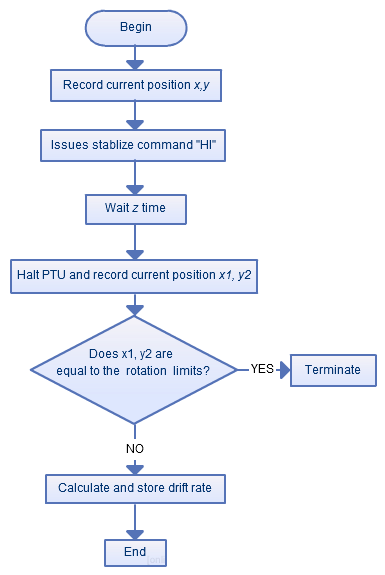
\includegraphics[scale=0.70]{./images/DriftRate}}
\caption{Drift rate calculation}
\label{fig:DriftRate}
\end{figure}

Since the time frame for this task to take place is specified in advance, there is a check to make sure that during the initial drift rate calculation procedure PTU doesn't hit its physical rotation limits. The logic is that if it did hit rotation limits, platform would not be drafting any further, however the time would be still moving forwards. We can not rely on that data from about the second position since we don't know how quickly rotation limits where hit. Hence we can not accurately determine the drift rate based on this data.

\subsection{Drift rate for the moving vehicle}
The drift rate calculation for the moving vehicle is a bit more complicate and requires information about the platform position in the space. The rover will be stopping from time to time to do a drift rate calibration. However it is very unlikely that when it stops position will be the same as it was the last time when calibration took place. To be able to calculate drift rate, while PTU is being stabilized and rover moved to a different place, we need to know current PTU orientation in the space (inclination angles of the chassis that PTU is mounted on). For this purpose inclinometer, mounted on the chassis, will be used to obtain current vehicle position. Knowing the inclination of the chassis and current PTU platform position we can find out difference between these two values which will be the drift rate. The algorithm for the drift rate calculation is presented on the figure ~\ref{fig:DriftRateInclinometer}

\begin{figure}[H]
\centering
\centerline{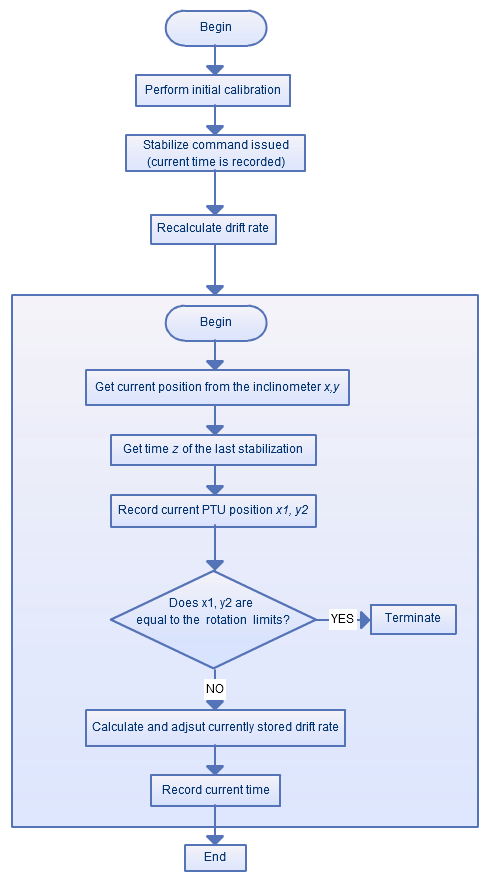
\includegraphics[scale=0.70]{./images/DriftRateInclinometer}}
\caption{Drift rate calculation for the moving vehicle}
\label{fig:DriftRateInclinometer}
\end{figure}

 